\documentclass{beamer}


% Automaton/graphs package
\usepackage{tikz}
\usetikzlibrary{automata,positioning,arrows.meta,petri}


%Information to be included in the title page:
\usetheme{AnnArbor}
\usecolortheme{beaver}

\title[YAFC]{Projet YAFC}
\subtitle{Yet Another Flight Controller}
\author[OYEZ]{Oussama Felfel \and
Yasmine Benhaddou\texorpdfstring{\\} \and
Elana Courtines \and
Zineb Moubarik}
\institute[UT3]{Université Paul Sabatier}
\date[01/12/2022]{1er Décembre 2022}
\logo{\includegraphics[height=1cm]{../logoUT3.png}}

\AtBeginSection[]
{
  \begin{frame}
    %\frametitle{Table of Contents}
    \tableofcontents[currentsection]
  \end{frame}
}



\begin{document}

\frame{\titlepage}


\section{Context, Objective}

\begin{frame}
    %\frametitle{Sample frame title}
    Yet Another Flight Controller (YAFC) is a project being held within the Computer Science Master at Université Paul Sabatier.

    \vspace*{5mm}

    Zhenyu Bai expressed their interest in drones. In particular for drones :
    \begin{itemize}
        \item that are cheap to produce ;
        \item physically basic ; 
        \item easily configurable.
    \end{itemize}
    
    \vspace*{5mm}

    The project thus aims to provide a functionnal drone that complies with the aforementioned critierias.
\end{frame}

\begin{frame}
    While the Flight Controller (FC) is the piece of software that controls the different physical components of the drone itself, the autopilot is what autonomously controls what the drone does.

    \vspace*{5mm}

    Today, completely functionnal and ready-to-use drones are expensive. But it is technically possible to produce cheap drones using or inspired by PixHawks.

\end{frame}

\section{Needs}

\begin{frame}
    
    From a provided functionnal drone frame, Zhenyu Bai expressed the need :
    \begin{itemize}
        \item to produce the Arduino code using PixHawks and PX4 ;
    \end{itemize}
    
    \vspace*{5mm}

    Subsequently, gradually, the following elements may be produced :

    \begin{itemize}
        \item the files to produce a custom-made PCB ;
        \item a custom-made FC inspired by PixHawks ;
    \end{itemize}
\end{frame}



\section{Organisation}
\subsection{Project Management}
\begin{frame}
    \begin{center}
        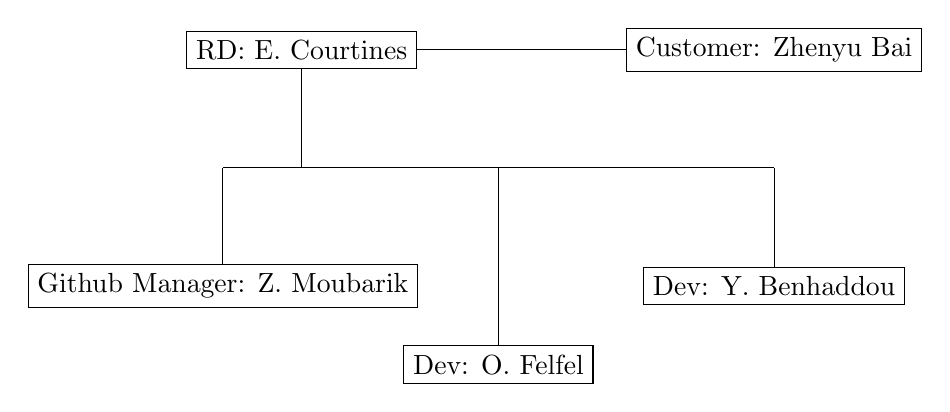
\begin{tikzpicture}
            \node [rectangle,draw] (rd) at (-2.5,0) {RD: E. Courtines};
            \node [rectangle,draw] (client) at (3.5,0) {Customer: Zhenyu Bai};
            \node [rectangle,draw] (l) at (-3.5,-3) {Github Manager: Z. Moubarik};
            \node [rectangle,draw] (m) at (0,-4) {Dev: O. Felfel};
            \node [rectangle,draw] (r) at (3.5,-3) {Dev: Y. Benhaddou};
            \node (link) at (0,-1.5) {};
            \node (aboveleft) at (-3.5,-1.5) {};
            \node (aboveright) at (3.5,-1.5) {};

            \path[-]
            (rd) edge (-2.5,-1.5)
            (link.center) edge (aboveleft.center)
            (link.center) edge (aboveright.center)
            (aboveleft.center) edge (l)
            (aboveright.center) edge (r)
            (link.center) edge (m)
            (rd) edge (client)
            ;

        \end{tikzpicture}
    \end{center}
\end{frame}

\begin{frame}
    \begin{minipage}{0.48\textwidth}
        Project Management Deliverables :
        \begin{itemize}
            \item Kick Off Meeting presentation and minutes (project Plan V0)
            \item Project Plan V1
            \item Project Plan V2
            \item Project Plan V3
            \item "Soutenance"
        \end{itemize}
    \end{minipage}
    \hfill
    \begin{minipage}{0.48\textwidth}
        Technical Deliverables :
        \begin{itemize}
            \item Archive containinig the Arduino code that uses PixHawks and PX4 ;
            \item Archive containinig all the required documents and files to reproduce a custom-made drone.
        \end{itemize}
    \end{minipage}
\end{frame}


\subsection{Development Management}
\begin{frame}
    A Github organisation has been created for the project : \href{https://github.com/OYEZ-YAFC}{https://github.com/OYEZ-YAFC}

    \vspace*{10mm}

    A private Repository will contain all of the code of the project. The Customer will be able to access it.

    \vspace*{10mm}

    While most of the code will be written in C, there will also be LaTeX and components description files.
\end{frame}



\subsection{Customer - Supplier Communication}
\begin{frame}
    Most of the communication will happen on Discord, while the important exchanges will be done by email.

    \vspace*{5mm}

    If needs be, the client will be able to submit issues directly on the Github Repository.
\end{frame}




\end{document}